
%%%%%%%%%%%%%%%%%%%%%%% file typeinst.tex %%%%%%%%%%%%%%%%%%%%%%%%%
%
% This is the LaTeX source for the instructions to authors using
% the LaTeX document class 'llncs.cls' for contributions to
% the Lecture Notes in Computer Sciences series.
% http://www.springer.com/lncs       Springer Heidelberg 2006/05/04
%
% It may be used as a template for your own input - copy it
% to a new file with a new name and use it as the basis
% for your article.
%
% NB: the document class 'llncs' has its own and detailed documentation, see
% ftp://ftp.springer.de/data/pubftp/pub/tex/latex/llncs/latex2e/llncsdoc.pdf
%
%%%%%%%%%%%%%%%%%%%%%%%%%%%%%%%%%%%%%%%%%%%%%%%%%%%%%%%%%%%%%%%%%%%


\documentclass[runningheads,a4paper]{llncs}

\usepackage{amssymb}
\setcounter{tocdepth}{3}
\usepackage{graphicx}

\usepackage{url}
\urldef{\mailsa}\path|{alfred.hofmann, ursula.barth, ingrid.haas, frank.holzwarth,|
\urldef{\mailsb}\path|anna.kramer, leonie.kunz, christine.reiss, nicole.sator,|
\urldef{\mailsc}\path|erika.siebert-cole, peter.strasser, lncs}@springer.com|    
\newcommand{\keywords}[1]{\par\addvspace\baselineskip
\noindent\keywordname\enspace\ignorespaces#1}

\begin{document}

\mainmatter  % start of an individual contribution

% TITLE 
\title{ Contextual Persuasion Modeling : How to Explain Intervention Tailoring to a Programmer }

% SHORT TITLE
\titlerunning{Contextual Persuasion Modeling}

% the name(s) of the author(s) follow(s) next
%
% NB: Chinese authors should write their first names(s) in front of
% their surnames. This ensures that the names appear correctly in
% the running heads and the author index.
%
\author{Tylar Murray
%\thanks{Please note that the LNCS Editorial assumes that all authors have used
%the western naming convention, with given names preceding surnames. This determines
%the structure of the names in the running heads and the author index.}%
\and Eric Hekler
\and Donna Spruijt-Metz
\and\\ Daniel E. Rivera
\and Andrew Raij
}

% SHORT TITLE (AGAIN)
\authorrunning{Contextual Persuasion Modeling}
% (feature abused for this document to repeat the title also on left hand pages)

% the affiliations are given next; don't give your e-mail address
% unless you accept that it will be published
\institute{University of South Florida, Arizona State University, University of Southern California, University of Central Florida\\
%Tiergartenstr. 17, 69121 Heidelberg, Germany\\
%\mailsa\\
%\mailsb\\
%\mailsc\\
%\url{http://www.springer.com/lncs}}
tylarmurray@mail.usf.edu
}

%
% NB: a more complex sample for affiliations and the mapping to the
% corresponding authors can be found in the file "llncs.dem"
% (search for the string "\mainmatter" where a contribution starts).
% "llncs.dem" accompanies the document class "llncs.cls".
%


% TODO: WHAT ARE THESE?
\toctitle{Lecture Notes in Computer Science}
\tocauthor{Authors' Instructions}
\maketitle


\begin{abstract}
TODO

\keywords{
  TODO
}
\end{abstract}

%%%%%%%%%%%%%%%%%%%%%%%%%%%%%%%%%%%
%%% %%% %%% PAPER START %%% %%% %%%
%%%%%%%%%%%%%%%%%%%%%%%%%%%%%%%%%%%
\section{Introduction}
A recent trend in the area of persuasive technology is the development of mHealth applications which aim to deliver better, smarter, and more effective interventions via mobile and wearable devices. 
One class of persuasive technologies with this aim is the “Just-In-Time Adaptive Intervention” or JiTAI which describes an intervention that adapts to an individual’s changing needs and circumstances to deliver tailored support at the time when it is most needed.

Thanks to great advances in wearable, mobile, and ubiquitous technologies an increasingly huge amount of data is now available to characterize the circumstances (aka context) of the subject.

Real-time monitoring of data to identify states of vulnerability or receptivity at any given moment is possible \cite{Hekler, Klasnja, Traver, & Hendriks, 2013}, but “a major gap exists between the technological capacity to deliver JITAIs and existing health behavior models.“ \cite{nahum2014}
Researchers theorize that an intervention which can tailor based on the user and context may be an elegant solution to empower self-management of unhealthy behaviors like substance abuse, overeating, sedentary behavior, and more \cite{nahum2014, Hekler, Patrick, & Michie, 2016}.
Proof-of-concept applications have demonstrated the ability to adapt interventions to users \cite{dallery2014optimizing, beck2010challenges} and context \cite{brailsford2010towards, collins2004}, but using current methods the complexity of the behavioral model underlying a JiTAI application grows exponentially as the complexity of the intervention design increases. 
Current behavioral theories focus on nomothetic and static insights that do not offer the granularity and specificity to support the full potential of JiTAIs\cite{riley2011health}.
The current development process for JiTAI-like persuasive technologies requires close collaboration between behavioral scientists and application developers as they struggle to code-ify the model from extant behavioral theories for each individual experiment.
The models used by a programmer to describe a “user” and the models used by behavioral scientists to describe a “subject”, have certain key differences which can complicate the process of JiTAI design.

In this work we present a hybridization of the two modeling paradigms designed to emphasize the strengths of each approach based on the recent work of Nahum-Shani et al. \cite{nahum2014}.
The following interdisciplinary language and concepts will help enable communication between developers and behavioral scientists, and these concepts may also form the foundation of an improved methodology for the development of persuasive technology interventions.
As a part of this set of interdisciplinary terms, we introduce the concept of a Computational Human Behavior Model (CHBM) to describe this new class of models which aim to satisfy the demands of persuasive technology.
The progression of behavioral science towards computational modeling has progressed more slowly than in other scientific domains because of the limited amount of detailed, time-intensive contextual and behavioral measures available.
SOME ARTICLE SOMEWHERE highlights the progression of scientific modeling from casual descriptive models to computational modeling as amount of data available to a domain increases, and the study of human behavior seems to be following this trend. \cite{THAT ONE ARTICLE}

Following definitions, we propose that by formalizing the CHBM underlying persuasive applications, it may be possible to create better behavioral theories, enable real-time ideographic optimization, facilitate more robust data analysis, and reduce application development time. 
In this section we present a look at how the concept of a CHBM might be applied to address open issues holding back JiTAIs and we highlight the remaining issues which must be addressed to make Just-in-Time Adaptive Interventions a reality.

\section{Selected Definitions}
In this section we present definitions and design considerations relevant to human-behavior modeling from a theory-agnostic standpoint so that different modeling paradigms can be described under a common foundation.
This set of definitions draws from both the area of HCI user-modeling and the extant paradigms of human behavior modeling in behavioral science in an attempt to synthesize a pragmatic language for use in the development of persuasive technology by behavioral scientists and application developers alike.
\subsection{Just-in-Time}
Nahum-Shani et al. summarize the cross-disciplinary concept of Just-in-Time (JIT) as “the effective provision of timely support, operationalized by offering the type of support needed, precisely when needed, in a way that minimizes waste (i.e., defined as anything that does not benefit the person) and accommodates the real-life setting in which support is needed.”
The primary focus of the JiT intervention approach is to attempt to intervene in the times when individuals are most vulnerable to negative behavior or receptive to positive change \cite{Ben-Zeev et al., 2014; King et al. 2013}, which may arise anytime throughout the day \cite{Fletcher, Tobias, & Wisher, 2007; Witkiewitz & Marlatt, 2004}.
Thus, for an intervention to be considered Just-in-Time (JiT), it must attempt to deliver an intervention immediately before or after an event associated with the target behavior. 
For example, a smoking cessation JiT intervention may deliver an intervention in response to increased craving.
It is important to note here that the term “event” is used to represent any exact set of circumstances over any predefined length of time.
The targeted event can therefore represent not only “behavioral events” (such as a jog, smoking a cigarette, commuting to work), but also an interval of availability \cite{???}, a “meaningful moment” \cite{???}, or any “optimal time” \cite{???} defined by a match between a set of observed datapoints and a set of datapoints which define the event archetype.

Though proof-of-concept studies have shown positive results delivering interventions just-in-time for ??? \cite{???}, “very limited behavioral research has been devoted to identifying markers of receptivity, and we have no robust models that can clarify how receptivity can shift as a function of continued exposure to specific types of support. [...] Much more work is needed in this domain.“ \cite{nahum2014}
subsection{adaptive}
For an intervention to be considered adaptive, it must utilize dynamic (time-varying) “information from the person (e.g., changes in psychological distress, response to an intervention, intervention adherence) [...] to make intervention decisions repeatedly in the course of the intervention (e.g., changing the type, dosage, or timing of intervention delivery).” \cite{nahum2014}

An adaptive intervention is one that responds in real-time to the changing needs of the participant by tailoring the intervention itself based on situational context or the recent behavioral history of a user. 
For example, a weight loss trial might attempt to remove soda from a participant’s diet and then move on to the next goal if the intervention was successful.
Similarly, consider the use of step goals to increase physical activity for an obese individual - the goals may start off at a realistic level (1000 steps/day) and then build up slowly as the individual’s ability progresses.
Lastly, consider “when s/he is around other people, providing certain types of support (e.g., feedback) might jeopardize the person’s privacy (De Costa et al., 2010).” \cite{nahum2014}

“With regard to opportunities for positive change, various learning and motivational theories highlight the importance of concepts such as shaping (i.e., training by reinforcing successively improving approximations of a desired behavior: Bouton, 2007; Ferster & Skinner, 1957) and teachable moments (i.e., a time when a person is more likely to internalize information and take action; Fisher, Piazza, & Roane, 2011; Murimi et al., 2014; Leist & Kristofco, 1990).“ \cite{nahum2014}
\subsection{individualized}
Nahum-Shani et al. define individualization as the “use of [static] information from the individual to make decisions about when, where and how to intervene.” \cite{nahum2014}
Thus, an intervention is individualized if “relatively stable information from the person (e.g., gender, baseline severity of symptoms) is used to make intervention-related decisions (e.g., to offer intervention package A or B)” \cite{nahum2014}
For example, a stress-relief intervention regimen may utilize relaxing music based on the subject’s favorite songs at study initialization, or a participant’s favorite color may be used as the basis for the user interface color palette.

One might consider a user’s manually applied application settings to be a (crude) form of individualization controlled by the user.
Allowing the user to specify their preferences reveals differences between users, which might be thought of as an expression of the user’s individual traits.

It is important to note that the static information used to tailor the intervention generally does not include the “personality” of the user.
Since the concept of personality has deep and complex roots in behavioral science, it may be considered separately as a special case of individualization based on established personality measures.
\subsection{personalized}
Personality is a long revered and reviled construct in psychology with many well-developed and validated measures, which are generally unutilized in the world of JiTAIs. 
Given that personality is (usually) considered a stable trait, an intervention application might be tailored before deploying based on a personality assessment.

...

Adapting to the user’s personality is therefore considered separate from the concept of an “Adaptive Intervention” which adapts according to situations and behaviors, and distinct from “intervention individualization”, which adapts the intervention regimen based on static variables not considered a part of existing theories of personality.
\subsection{JiTAIs}
Nahum-Shani et al. “conceptualize the JITAI as an intervention design that uses a dynamic form of individualization to operationalize the provision of JIT support. Specifically, JITAIs operationalize the individualization of the selection and delivery of intervention options based on ongoing assessments of the individual’s state and ecological context, with the goal to offer the right type of support precisely when, and only when, the person is in a state of vulnerability/opportunity and receptivity” /cite{nahum2014}.
Thus, JiTAIs are interventions which attempt to leverage the benefits of being both “adaptive”, and “just-in-time”. 

JiTAIs are an active area of research spanning nearly all applications of persuasive mHealth technology, including:
physical activity (King et al. 2013; Consolvo et al. 2008), 
drug abuse (Dennis, Scott, Funk, & Nicholson, 2014), 
alcohol use (Witkiewitz et al., 2014; Gustafson et al., 2014), 
smoking cessation (Riley, Obermayer, & Jean-Mary, 2008), 
obesity/weight management (Patrick et al., 2009), 
and mental illnesses (Ben-Zeev et al., 2014).

Though JiTAIs offer much for the future of preventative medicine and behavior change, more work is needed to make JiTAIs a reality.
“Current health behavior theories and related empirical evidence paint a largely static picture of human behavior, cognition and emotions; they fail to capture the dynamic processes underlying the emergence of a vulnerable state or the adoption and maintenance of healthy behaviors (Spruijt-Metz et al., under review). Even dynamic models that acknowledge the role of episodic factors in health behavior processes (e.g., the dynamic model of relapse; Witkiewitz & Marlatt, 2004) do not specify the temporal nature of each factor in a way that informs when and how to intervene. Although many health behavioral models acknowledge individual differences in response to treatment, in most cases these models can only inform the most basic form of individualization (i.e., they use single time point factors like age, gender, or baseline symptom severity to make intervention decisions) rather than the dynamic individualization required to operationalize JIT support. Finally, existing intervention models often adopt a one-size-fits-all approach to intervention provision (Drotar & Lemanek, 2001; Marcus et al., 2000; Sorensen, Emmons, Hunt, & Johnston, 1998), failing to provide actionable insights with regard to the various elements of individualization articulated above.” \cite{nahum2014}
Thus, novel modeling architectures and methodologies may be needed to overcome some of these shortcomings of existing JiTAI applications.
\subsection{Human Behavior Model}
In principle, persuasive interventions are based on an underlying  model of the subject and their behavior. 
This Human Behavior Model (HBM) could be implicitly or explicitly defined.
An implicit model is one that is expressed through the behavior of the designed system. 
For instance, an intervention which delivers eating-behavior guidelines daily at noon has an implicit user model which states that users are awake and likely to eat soon at midday.
The intervention design reveals the underlying model.

In contrast, an explicit model  defines the user model underlying the operating principles of the intervention. This model is often based on the operationalization of a particular theory (or theories) which have guided the design of the intervention.

The distinction between the terms model and theory as used here is an important one; in existing literature there exists some overlap and ambiguity regarding the use of the terms so we provide short definitions here.

The preferred definition of a theory given by Davis, Campbell, Hildon, Hobbs, and Michie \cite{davis2014} states that a theory is “a set of concepts and/or statements [...] that accounts for what is known, and explains and predicts phenomena.”
A theory describes the causality of events, but does not provide quantitative predictions.

The term model as used here is best defined by Spruij-Metz and Nilsen \cite{spruijtmetz2014} as an empirical, quantifiable, and testable construction which may be informed by multiple theories.

Thus it can be said that a theory is a conceptualization which may inform a model, whereas a model is a mathematical construction that quantifiably defines a system.
As an example, consider the Theory of Planned Behavior \cite{Bandura???} as the primary driving theory behind Rivera/Dong/??? \cite{???} et al.’s model of the human system which puts a particular focus on gestational weight gain/smoking/???.

Theories paired with causal descriptive models provide means to conceptualize and predict human behaviors.
Such causal descriptive models inform our understanding of the human system part-by-part, but they do not form a pragmatic interconnected picture of how the human system translates past history and current context into behaviors.  


The majority of extant approaches utilize nomothetic models focused on constructs that remain relatively static over time such as demographic factors, psychiatric diagnoses, and patterns of high-risk behavior \cite{Spruijt-Metz, Nilsen, & Pavel, 2014}.
A JiTAI application requires that very specific details are given about nature and dynamics of the influence of interventions, the internalization of contextual information, and subject behaviors.
If these details are not given, then simple assumptions are used to fill in the gaps based on the developer’s intuition (or oversight) and implicit modeling assumptions are added.
In short, extant Human Behavior Models are insufficiently detailed to fully inform a modern digital health intervention \cite{riley2011}.
The (often poorly documented) assumptions injected or overlooked as the implicit model materializes may significantly influence the power of a JiTAI, and current literature provides little guidance regarding the model structure or predictions needed to scientifically inform JiTAI development.

It stands to reason that more detailed models and more realistic modeling assumptions may lead to better JiTAIs, but the process of creating models of human behavior at the level of detail needed requires a paradigm shift.
Methods for translating between existing causal-descriptive models and dynamical systems formulations have been explored for TODO: APPLICATIONS \cite{csel?}. 
These formulations, however, also include details and concepts which --- though they are usually overlooked by existing behavioral models --- can represent important aspects of behavioral theory.
Including these concepts requires that more behavioral science must be injected into model, making this is a task which requires both detailed knowledge of the applicable behavioral science as well as familiarity with systems modeling.
\subsection{Computational Human Behavior Model}
A Computational Human Behavior Model (CHBM) is defined here as an explicit, mathematical description of how context is transformed into a behavioral outcome through the internal state of the human system.
This definition includes no constraints on the mathematics that govern variable relationships, the theories underlying the CHBM, or on the way internal state is abstracted.
CHBMs are a subclass of Human Behavior Models which obey a set of conventions put in place to improve the utility of CHBMs with regards to JiTAIs and persuasive technology in general.

The mathematical definition of a CHBM can provide idiographic insight, i.e. it may be used to forecast behaviors given a context history and the anticipated future context or predict behavioral phenomenon for a particular individual, but a CHBM should also provide nomothetic abstraction(s) which allows researchers to anticipate the general behavior of a population.
Statistical models trained on data do qualify as CHBMs in that they can define the relationships between state and context, but typically do not incorporate a logical abstraction of cognition and instead treat the internal state as a “black box”.
This abstraction is essential when considering the process of JiTAI design, since the search-space available to a JiTAI designer can only be approached through heuristics guided by an understanding of how the human system will generally behave under given conditions.

\subsection{HBM info-flow graph}
There are countless approaches to systems modeling, but concepts and methods ought to be incorporated and fused when possible in their application to behavioral science.
The following specification will allow for the formal description of an HBM, providing a standard approach to describing, designing, and visualizing human behavior models for personal forecasting .

For the representation of an HBM, we define a network graph to describe the flow of information between nodes.
We argue that the most intuitive representation in this case is one which uses a directed graph wherein edge arrows represent the flow of information between nodes.
Thus, a directed graph edge from node A to node B indicates that information flows from node A into node B. 

\begin{centering}
  $A => B$\\
  \small{Graph 1: Can be read as "A influences B", "A informs B", or similar.}
\end{centering}
  
This choice of notation is in agreement with graphs used in information theory, communications models, and behavioral science.
In contrast, some graphing paradigms (such as probabilistic graphical models and software design) prefer to use notation wherein an edge is used to represent dependency.
In these paradigms edges may be read from tail to head as "depends on" or similar.

While the network graph shows the connectivity of a model, it fails to indicate the meaning of each connection.
In the majority of existing applications, the mathematical form of the relationship is implied or else it is neglected completely.
For instance, path diagrams from the behavioral sciences frequently denote dependence and do not specify functional form.
Adding even further to the confusion is the notion that these graphs are often developed using different statistical analyses which may make other assumptions about the functional definition of inter-variate dependency.
The most common analyses assess linear relationships between variables, and thus it is perhaps reasonable to assume that this is the intention of most authors.
Assuming this is the case we can return to our simplistic example in Graph 1 and interpret the implied relationship as:

\begin{centering}
$B(t) = coeff_{ab}A(t) + const_b$\\
\small{Equation 1: $coeff_{ab}$ represents the correlation coefficient which relates A to B, and $const_b$ represents a scalar constant.}
\end{centering}

For nodes with multiple inflow edges, such as node B in the following graph:

\begin{centering}
$A => B <= C => D$\\
\small{Graph 2: B depends on nodes A and C.}
\end{centering}

Continuing with our our assumption that node interrelations act as linear sums, the resulting formulation is simply a sum of the inflows:

\begin{centering}
$B(t) = coeff_{ab}A(t) + coeff_{cb}C(t) + const_b$\\
\small{Equation 2: Combining multiple inflows via sum is referred to as the superposition principle and is the defining characteristic of linear systems (not to be confused with this linear formulation)}
\end{centering}

Using this formulation, the general form of our HBM is expressed via the network graph alone (perhaps along with a statement about what edges mean).
To express an ideographic implementation of this general model, we must also include a table of coefficient values. 

This linear, homogeneous-graph representation is useful, but also very limited.
One important feature which this formulation does not take into account is the dynamics of the relationship.
This is very important for human behavior modeling because the variables in a HBM will often respond with some delay.
This assumption is fine for many applications, but we argue that this is a very poor assumption for human behavior models. What if A is influenced by B but there is some lag before the effect manifests?
What if A is influenced by B, but only if B is above some threshold value? What if A is influenced by the rate of change in B rather than the value of B itself? All of these scenarios cannot be expressed using this simple linear relationship. 

To resolve some of these issues, a differential equations can be used to describe the relationship between variables as described by Dong et al.\cite{dong2012dynamical}. 
Using the differential formulation our equation for B in Graph 1 becomes:

\begin{centering}
$B(t) = coeff_{ab}A(t-\theta_{ab}) - \tau_{b}\frac{dB}{dt} + const$\\
\end{centering}

Just as before, our general model is not expressed entirely through the graph, and an ideographic example is specified by providing table of coefficient values.
Our table is now quite a bit larger, but these coefficients have meaningful definitions which relate to our theory.
While this formulation offers a huge improvement over the linear formulation, we can still imagine relationships which it cannot express.
Thus, perhaps a graph-wide assumption that each edge represents a differential equation is not general enough for our HBM specification. 

It should be noted at this point that although the linear formulation is too simple to express the dynamics of the differential formulation, the differential formulation is capable of expressing linear relationships.
This is accomplished by setting coefficients of dynamical components to 0.
One might think, then, that there is some general formula which could express any functional form, and that this form should be used to express the relationships between variables in our HBM graphs.
While such formulations do exist (such as Taylor or Fourier series approximations or even ANN-based relations), this usage tends to make the model difficult to understand and to simulate with.
Indeed, linear and differential formulations are in such widespread use because of the relative ease with which we can understand and solve them. 
% An additional problem raised by this approach is that of redundant formulations.
% As a formulation grows in complexity there are an increasing number of solutions which may fit our requirements equally well, creating more potential for confusion between researchers.
% Formulations could even subvert the "arrow direction" by drawing information contrary to our original choice of notation.
% The graph can then no longer be considered a directed graph, and the meaning of an edge becomes less clear.
Additionally, the table of coefficients needed to express an ideographic case of the model quickly becomes prohibitively large, and the effect of each coefficient on the outcome is not intuitively meaningful.

Let us now consider the case where a graph-wide assumption is \emph{NOT} made.
That is, we will specify the functional form of each node individually so that each edge on the graph may be linear in form while another may be differential.
This has the benefit of allowing for both complex relationships between variables as well as simplistic ones.
In this way one could craft a model in which two variables are linearly related and a third is dependent on the variance of another variable (a particularly odd formulation, but one which is relevant to behavioral theory).
Unfortunately, this approach also means that a table of formulations must now be included with our graph to show the meaning of each edge in the graph.
Consider for example the table below for Graph 2:

\begin{centering}
  \begin{tabular}{ | l | l | l |}
      \hline
      node & formulation \\ \hline
      B & $coeff_{ab}A(t) + coeff_{cb}C(t) + cosnst_b$  \\ \hline
      D & $coeff_{cd}C(t-\theta_{cd}) - \tau_{d}\frac{dD}{dt} + const_d$ \\ \hline
  \end{tabular}
  
  Table 1: an example formulation table for Graph 2, showing a linear and first-order differential equation relations between constructs, respectively.
\end{centering}

If a fixed number of functional forms is adhered to, the graph can be made to visually represent these functional forms through the use of different node icon shapes. 
This approach quickly begins to resemble applications which use flow-based programming. 
Indeed, they are quite similar in their approach, and the specification of a HBM is quite similar to the writing of a program.

Note also that a node can set any arbitrary formulation if needed. 
This is the least desirable situation, since the meaning of an inflow to each node even more convoluted. 
Though this usage reduces the ability of the graph to reduce processing load on the user through abstraction, there may be some cases where this type of formulation is desirable. 
Consider the following graph and formulation table:

\begin{centering}
$A => B <= C => D => E$\\
Graph 3: A and C are environmental inflows, D is an internal state variable, and B and D are behavioral outputs.
\end{centering}

\begin{centering}
  \begin{tabular}{ | l | l | l |}
      \hline
      node & formulation \\ \hline
      B & $coeff_{ab}A(t) + coeff_{cb}sqrt(C(t)) + const_b$ \\ \hline
      D & $coeff_{cd}C(t-\theta_{cd}) - \tau_{d}\frac{dD}{dt} + const_{d}$ \\ \hline
      E & $coeff_{de}D(t) + const_{e}$ \\ \hline
  \end{tabular}

  Table 2: an example formulation table for Graph 3 showing a custom, differential, and linear relationships, respectively.
\end{centering}

In conclusion, we propose that an HBM should be specified using the following rules:

\begin{enumerate}
  \item use a graph-wide formula assumption if possible, else specify formulations for each node individually
  \item when choosing a formulation, consistency between nodes is most important
  \item when choosing a formulation, simplicity and clarity is second only to consistency
\end{enumerate}
  
Thus a HBM specification must include:
\begin{enumerate}
  \item An information flow graph
  \item either: a graph-wide formulaic assumption or a formulation table 
\end{enumerate}

\subsection{User Interface Design for HBM-builder }
The flow chart shown in figure \ref{HBM-build-process} represents the movement of a user through the process of building an HBM using the proposed information flow graph specification.

\begin{figure}[!t]
  \centering
  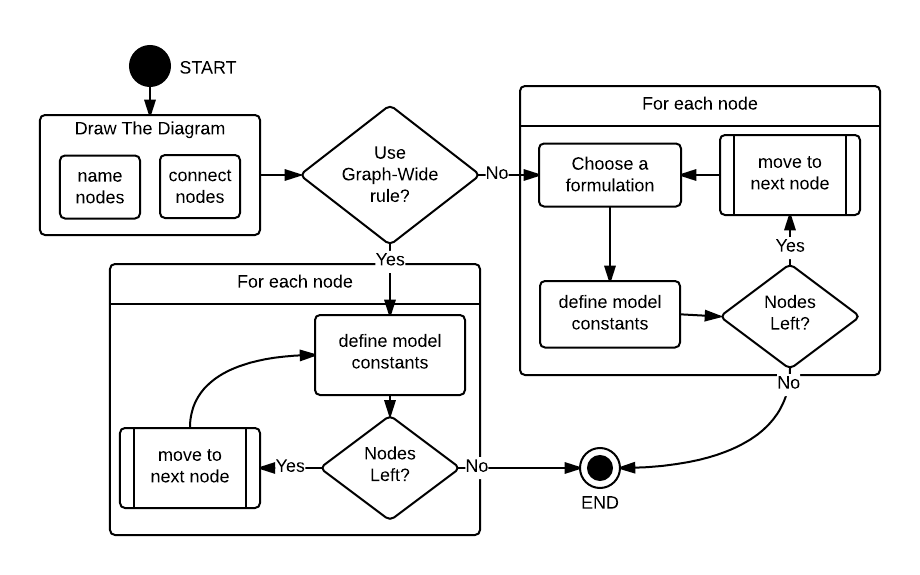
\includegraphics[width=0.9\columnwidth]{img/HBM-build-process}
  \caption{Flow chart depicting the process of building a graphical HBM.}
  \label{HBM-build-process}
\end{figure}

It is important to note that the process of building is pseudo-linear; users will likely want to jump back to an arbitrary point and as the model takes shape. 
As the user moves through the process, they will re-assess the meaning of variables and connections and their model will solidify. 
UI for an HBM-building tool should enable easy backtracking and should work to provide feedback on the characteristics of the model early. 
Keeping the non-linearity of this process in mind, we will now walk through the diagram and address design considerations for each part of the process.

\subsubsection{Draw the Diagram}
This task involves the creation and connecting of all nodes in the diagram. 
Nodes and their connections should be primarily based in theory, so a user should be able to build a first draft of their model with little feedback. 
Once the formulas for each node have been specified, however, it is likely that the user will want to return to this step and reassess the network. 
Several paradigms diagram-drawing have been well tested, but there are essentially two prevailing options:
1) drag-and-drop node creation with drag-to-connect edges, and 2) textual ``diagram specification language'' (DSL).

Drag-and-drop modeling has the benefit of being intuitive, but nodes can be difficult to position to reduce edge overlap leading to users often distracted trying to optimize the layout.

The use of a DSL can be much faster than mouse-reliant alternatives, and also has the benefit that searching/finding nodes for modification is as easy as textual search of the DSL.
On the other hand, DSL parsing errors can be a major source of confusion and users may be more frustrated as they attempt to master the markup language.


\subsubsection{Use Graph-Wide Rule?}
This choice can come before or after the initial drawing of the graph, since it is likely the user has a graph-wide assumption in mind when starting the process. 
This choice determines whether or not the interface for specifying nodes individually is shown, so it is logical to think of the "none", "node-specific", or "node-unique" option as one of the choices available here. 
As an example, some graph-wide rules which may be implemented include a probabilistic graphical network, linear sum assumption, fluid-flow analogy.

If a graph-wide rule is set, the formulation section for each node should show as locked to the rule's respective formulation. 
Editing an individual node's formulation will disable the graph-wide rule, and should require confirmation from the user. 
The interface for choosing one of these rules may be as simple as a select-option box or may include a detailed rule description and example. 
An additional feature which may be useful is to allow for user-defined graph-wide rules. 
In this case, users might choose "create new rule" and an interface to allow users to edit and save graph-wide rules is needed.

% \subsubsection{For Each Node}
% 
% Items encapsulated by the "for each node" swim-lanes must be executed for each node in the graph. 
% The graph-wide-rule-yes case differs from the graph-wide-rule-no case only in that the graph-wide-rule-no case requires the additional step of setting the formulation at each node.

\subsubsection{Choose a Formulation}
This item is identical to the graph-wide rule choice, except that it applies only to a single node. Similar design considerations apply, and user-defined choice is even more important at this scale.

\subsubsection{Define Model Constants}
The general solution of an HBM does not require definition of the constants, but a simulation cannot be run until some numerical value is assumed. 
These constants often have theoretical significance in that they often have meaningful influence upon system behavior. 
Scaling-coefficients, for instance allow for relative weighting of each inflow. 
Similarly, the coefficients of a dynamical equation define how quickly variables react to a change ``upstream''.
UI for setting these constants could be as simple as a numerical input for each coefficient's name, but additional model details provided here may be of great benefit to the model designer. 

First, UI should include equation-specific descriptions of the constants whenever possible. This means that a separate UI for each formulation type is necessary. 
Second, adjustment of coefficients would ideally show changes in the dynamics of a node's value in real-time. 
This can take the form of a time-series chart of the selected node's numerical value over time along with (editable) time-series for the inflows. 
Adjustment of these inflow series may also take a number of different forms. 
Third, model creators may want to set these coefficients in three different ways: 
\paragraph{Set the coefficient value to a constant}
All simulations derived from this general solution will have this exact value.

\paragraph{Set a probability distribution for the coefficient}
Simulations derived from this general solution will select a numerical value based on the given distribution. 
This distribution may be learned from a training dataset, or bounds may be set for later training. 

\paragraph{Leave the variable unbounded and assume a flat probability distribution}
This selection is identical to option 2 with a flat distribution from -infinity to +infinity, but may deserve special inclusion due to the comparatively low complexity (making this option appealing for novice users).

These different ways of defining coefficients in a HBM become significant when it is time to run simulations and compare model results to real data. 
Last, model creators may want to use a measured value to set the value of these coefficients. In this way, one measured input (in real life), such as big-5 personality type, can be used to set the value of multiple coefficients across different variables in the model.

% \subsubsection{Nodes Left?}
% %This is the most simple element of the flowchart. 
% No if there are unspecified nodes remaining, yes if all are complete. 
% It should be left to the user to confirm model-completeness, however, since a great deal of model-tweaking is likely now that simulation results can be displayed.
% 
% \subsubsection{Next Node}
% Progression downstream through the model should be relatively straightforward in the case of tree-like models, but feedback loops can cause issues here. 
% Perhaps the best paradigm here is to progress as naturally as possible, but allow the user to over-ride and select any node. 
% This interaction mode will also be needed to allow for later model-tweaking. 


A distinguishing feature of a CHBM is the separation of environmental \emph{context}, internal \emph{state}, and \emph{behaviors}.
In reality, an individual represents an inseparable component within the larger environment, but this simplification segments out the human system for definition.

Dey et al (2001) performed an extensive literature search to define an agent’s context as: “any information that can be used to characterize the situation of entities (i.e., whether a person, place, or object) that are considered relevant to the interaction between a user and an application, including the user and the application themselves. Context is typically the location, identity, and state of people, groups, and computational and physical objects.” 
In most cases, it is sufficient to define context as a set of selected information from the environment available for inflow into the human system, but contextual information from the environment may be summarized and represented in countless ways, depending on the theories used to inform the model.
In the real world, consider this to be everything that is observed by the senses. 
Some of this information will alter the internal state of the human system, but some may not. 
The set of internal state variables which define the inner workings of the human system are dependent only on past states and the current context. 
In the real world, internal state includes all information stored in the chemical and physical  arrangement of our bodies. 
In order to make the model tractable, the mass of information is summarized into a set of meaningful constructs.
Behavior can be defined in many ways, but in a CHBM behavior is defined as any flow of information out of the human system and into the environment.
Information flowing into a CHBM comes from the environment around an individual (the context) as an inflow which is independent of the individual’s state in this instant.
Similarly, information flowing out of a CHBM (as behaviors) represents actions the individual is taking to impact the environment.

In summary, a Computational Human Behavior Model (CHBM) should have: 1) a set of context, state, and behavior variables, 2) a set of computations which define behavior variables as a function of state which is itself a function of context, 3) a logical abstraction which allows researchers to internalize the model’s behavior such that they may be better able to estimate control of the human system in general, and lastly 4) guidelines regarding the applicable population and time-scale of the CHBM (i.e. in what populations is the CHBM most/least valid, and at what time-scale can the CHBM simulate realistic predictions?). 
On this last point it should be noted that while a CHBM should strive to be as broadly applicable as possible, this inevitably comes at the cost of increased complexity which can make the CHBM’s nomothetic abstraction(s) intractable; there is a balance to be struck between a CHBM’s inclusivity and the clarity of the abstraction.
\section{benefits of CHBM-enabled JiTAIs}
This section discusses the utility of a CHBM throughout the lifecycle of a JiTAI application.
Hypothetical situations are posed to highlight the potential value of CHBM use in the JiTAI development process and show open challenges through establishment of a target user group model, application design, application implementation, data analysis, model personalization, and model iteration.

Existing methods for modeling behavior change are limited in their utility for the average software developer, but a mathematical formulation of the human system’s behavior allows developers to utilize existing methods from other engineering domains.

\subsection{a priori CHBMs}
Prior to development of a JiTAI, a mental model of the target user group is established.
This a priori model represents the researcher’s understanding of the user group, and the design of the intervention utilizes the model in order to predict user actions.
This level of detail to which this model is documented varies greatly between applications, and in some cases the causal descriptive model has little grounding in existing behavioral theory \cite{prestwich2014does}.

% research has (NOT?) indicated that persuasive applications with a firm basis in theory have been found to be more effective \cite{???}.
% “Establishing a scientific model is an important step in constructing behavioral interventions (Collins, Murphy, & Bierman, 2004).” \cite{nahum2014}

Nevertheless, a vague description of expected user behaviors and interactions with the persuasive technology still represents a user model.
Existing JiTAI-like applications may not have a CHBM, but they always (sometimes informally) imply a HBM.
This section highlights the benefits of defining a CHBM explicitly, rather than relying on implicit behavioral theory.
\paragraph{Model Building}
When model-building for a JiTAI, the planned system and underlying model of human behavior becomes very complicated, and user responses may be difficult to predict through thought experiments.
Without a concrete framework to describe the model, user behavior becomes oversimplified, giving an even less accurate picture of the complex human system.
When a model is under-developed, the application development process will open unaddressed questions and simple assumptions will be made.
For instance, delivery of an intervention may be limited to the waking hours or to the weekdays, but this will not be reflected in the described user model.
The mismatch between the documented theoretical model and the actually implemented model further muddle the process of study replication and analysis.

In addition to those assumptions knowingly made by application developers, causal descriptive modeling often contains implicit assumptions which are easily overlooked.
For instance, the delay between a cause and effect is frequently neglected --- that is: how quickly does a participant’s behavior respond to an intervention?
The process of defining a more detailed a priori model itself can lead to new insights and research questions by eliminating these oversights and forcing critical thinking on the assumptions being made /cite{Erik/Donna?}.

% TODO: expand on how dynamical modeling yields insights/research questions: 
% The use of these interventions, particularly in context, forces far more careful description of exactly when, where, and how an intervention might produce an effect and, equally as important, exactly when, where and how an intervention will NOT produce an effect. We might intentionally ask for “outside of the skin” factors such as times, locations, situations and internal states that dictate the boundary conditions on when a  particular causal relationship will be observable or not (Hovell, Wahlgren, & Adams, 2009).  We might also need to discriminate on different “within the skin” attributes that would also define success such as gender, ethnicity, preferences (e.g., while research is increasingly exploring the utility of consuming protein from insects, cultural issues and individual differences make this solution for reducing our collective carbon footprint almost impossible to implement with some groups; Hovell et al. 2009).  These discriminations become even more important when time is taken into account as behavior, “outside the skin” and “inside the skin” factors can all vary together over time (Hovell et al. 2009). This results in clear discrimination of the boundary conditions on when an intervention might work or not, or perhaps only manifest after achieving some largely critical “tipping point,” or wear off after habituation, can further be specified and thought through (Resnicow & Page, 2008; Hekler, et al 2016).

% Beyond the discriminations, there are also a wide range of irrelevant factors that can vary that will not influence the cause and effect relationship(s) under study. It might be believed, for example, that a particular intervention will work the same for men and women.  If that is the case, then having both women and men in the study is useful information  as it supports examining if this “irrelevancy” is truly irrelevant.  

\paragraph{Intervention Design}
When designing intervention options for a JiTAI application, researchers will consider how an intervention influences the subject in the context of the chosen user model.
When using a CHBM, this means quantifying the intervention’s effect on user context.
For instance, consider an intervention which provides information about the health repercussions of sedentary behavior.
Assuming our CHBM uses an adaptation of the Theory of Planned Behavior \cite{Bandura???}, this intervention targets “behavioral belief” regarding sedentary behavior.
Since “behavioral belief” is part of the internal state and the intervention should be defined as part of the user’s context, a context variable should be included in our model to represent external influences on “behavioral belief” from the environment.
After defining the expected effect of an intervention, the CHBM can then be used to predict a detailed account of user response.
The use of simulations such as this in the process of designing controls is well-explored in many other areas, but is nearly unheard of in behavioral science.
This is in part due to the prevalence of abstract causal descriptive models and the novelty of CHBMs, but there remain several important issues which have not yet been addressed.
First, the definition of an intervention’s effect on a user is a subjective process of quantifying qualities which currently have no point of reference.
That is: how is one to know what amount of “behavioral belief” a given “sedentary activity fact intervention” imparts?
Guidelines for estimating these values should become more clear after further precedent has been set, but no standards yet exist.
Second, the running of a single simulation implies a generically applicable user model, but in reality there are likely to be multiple different responses to a single intervention which may depend on on other contextual variables. 
In order to get a more realistic look at user responses to an intervention, many simulations with varying parameters set to match the expectations of the researchers should be run and analyzed; this would require a CHBM simulation software suite that does not yet exist.
% Third… ?

CHBM benefits: 
By using a CHBM with dynamical equations, the dynamics of relationships between variables can be explicitly described as a part of the model.
The use of an explicit a priori model for intervention design helps researchers formulate research questions and design experiments in a concrete, testable fashion.
This additional detail needed to define a CHBM removes post-design modeling assumptions and overlooked details that can dilute the underlying behavioral theory or invalidate study results.
The process of defining a CHBM itself can lead to new insights and research questions which are of particular interest to JiTAI design and are almost entirely unaddressed by existing theory.

Open questions:
The process of defining a CHBM requires detailed knowledge of both the underlying behavioral theory and the mathematics. Relatively few researchers today possess the necessary skillset, especially when considering the use of dynamical systems equations.
Modeling software to provide abstraction of the mathematical complexity exists for other engineering domains, but software is not directly applicable to the problem of CHBM development. %TODO how?
Software for running simulations to test the function of an a priori CHBM is non-existent, and standards for describing models, simulations, and results in this domain are not established.
Methodologies for creating an a priori CHBM are not fully established, and mappings from existing causal descriptive models (like CSEL’s fluid-flow analogy) may be model-dependent.

\subsection{CHBMs at Run-time}
In this section methods in which CHBMs may be used in the persuasive technology itself are discussed. 
Options include model-based intervention optimization, timing, and online ideographic modeling.

% the trouble with decision rules
A crucial step in the development of a persuasive technology today is to establish a set of "decision rules" based on behavioral theory which codify the circumstances in which an intervention should or should not be delivered.
For instance, an intervention might be delivered only during the daytime, right before a meal, only in a particular location, or in response to a behavioral event such as cigarette use.
Establishing a set of decision rules for a small number of conditions is feasible for a simple intervention, but as the number of conditions increases the number of rules required increases combinatorially.
Even worse, when making use of adaptive interventions this set of rules must be expanded even further to map between all possible contexts and intervention permutations.
Relying on simple decision rules loosely guided by existing theory to define the optimization of intervention delivery to control a complex system inevitably leads to under-optimized interventions, over-simplified models, and weakened data.
An additional problem with this approach is the use of a binary state (i.e. rule satisfied or not) to optimize delivery over a continuous time.
Consider a decision rule which is coincidentally satisfied for the entire first day of the study, and unsatisfied for the rest of the two-week study.

* Should the intervention be delivered on the first day continuously, on some interval, or randomly spread throughout the first day?
* Should no intervention be delivered for the remainder of the two weeks while the rule is not satisfied?
* Should some minimum number of interventions per day should be spread randomly or applied at particular times?
* Should there be a secondary fallback criterion if the primary rule is not satisfied?

The rules which govern the behavior in this case become part of the theory underlying the application and are clumsily expressed as decision rules.
In contrast, optimization of intervention delivery using a CHBM can be done algorithmically to minimize the area between the desired and observed target behavior.

Assuming that a CHBM has been formulated by behavioral scientists prior to implementation of the designed application, the software can directly make use of the CHBM to model the user.
Because CHBMs are computational in nature, prediction of behavior is possible given information about the user’s present and future context.
Furthermore, because the behaviors in computational models are quantitative, an application could search available intervention options to find one which produces the ideal amount of a target behavior.
That is, given three intervention options (A, B, C) with known effect on user context, the model can be run at t+1 for each option, and the optimum result can be chosen.
Methods for model predictive control are a well studied topic of control systems engineering, but many methods cannot be applied to generic formulations (such as the CHBM specification).
Without a constrained form to guide optimization, all possible options must be explored with equal feasibility in a brute-force search.
With sufficient computational power this is effective for simple problems, but this approach becomes increasingly infeasible as the number of options and the number of future steps to be considered increase.
If the functional form describing variable relationships is constrained appropriately, however, mathematical optimizations methods can greatly simplify this problem.
Applications of model-predictive control over intervention delivery have been explored for gestational weight gain \cite{dong2013hybrid, dong2014hybrid}, smoking cessation \cite{Timms2014hybrid}, and fibromyalgia treatment \cite{Deshpande2014optimized} by limiting the functional form of the CHBM specification to a differential equation based on a fluid-flow analogy.
In this way, application creators can implement software utilizing the advanced understanding of behavioral science described by the CHBM, without direct knowledge of the underlying behavioral science.

Methods of optimizing the timing and adaption of interventions thus far have assumed that the effect of interventions is well known a priori.
However, real-life users may respond very differently from the generalized model and personal ideographic models are not yet a feasible solution.
In order to optimize intervention delivery given a set of unknown interventions, an online learning has been proposed /cite{Luis???}.
In theory, a similar approach may be capable of producing a ideographic models of subjects which can then be generalized to improve understanding of the behavioral theory.

CHBM benefits:
Using a CHBM enables the use of optimization algorithms instead of decision rules. This change is needed to express the complexity necessary to effectively control target behaviors in the human system.
CHBMs can be adapted to fit a user's needs at run-time, establishing an idiographic model of each subject from the generalized CHBM.

challenges:
Optimization of intervention delivery can be computationally expensive unless the functional form of modelling is restricted, and it is not yet clear what formulations are most appropriate for behavioral construct relationships.
% ??? more ???

\subsection{CHBMs Post-Study}
Another rising challenge for persuasive technology researchers is the increasing complexity of data analysis methods needed to handle large amounts of "in the wild" data.
Techniques designed to simplify construct relationships using statistical inferences between distinct groups of measurements cannot address emerging research questions which span the full spectrum of subject demographics, situational context, and time-scale. 
Contemporary approaches apply data mining and machine learning techniques to fit more advanced models to study data and identify key factors, but findings revealed in these exercises can be difficult to generalize and interpret.
For example, “even if empirical evidence suggests that a given factor (e.g., psychological distress) marks state of vulnerability to a specific proximal outcome (e.g., it is highly predictive of poor state coping capacity), there is often insufficient empirical evidence concerning the cut-point of this factor that can inform the selection of one intervention option over another.” \cite{nahum2014}.
A shift in behavioral research from a focus on relationships between specific variables under specific conditions towards more generalizable hypotheses seems to have begun. 
This shift is being ushered in by researchers working with persuasive technologies who are looking for practical applications and easy-to-reproduce models of the human system.
By using a model as the hypothesis of an experiment rather than focusing solely on a particular relationship between two variables in specific conditions, research findings can be generalized more easily to practical persuasive applications.
Methods for evaluating models, rather than evaluating correlation between two variables should be increasingly focused upon in the analysis of behavioral data.
While analysis of correlation between variables looks at the statistical relationship between groups of data points, the evaluation of a model involves comparing the experimental data to the predictions of the model.
Thanks to advances in wearable sensors and mobile technology, models are able to predict behavioral outcomes from detailed contextual information collected in the study.

%TODO: include graphic?

CHBMs can be used with contextual data to produce a time series of expected behavioral outcomes throughout the study.
The simulated "theoretical data" can then be directly compared to the "observed data" to observe how the theory differs from the reality.
The process of comparing theoretical predictions to empirical data can be repeated with simulations from alternate theories and a goodness-of-fit metric can be used to evaluate the hypothesis against alternatives.
Additionally, unification of existing behavioral models into this common paradigm might enable better collaboration between proponents of different theories.

CHBM benefits:
Through the use of CHBMs, analysis of experimental data can shift focus from individual construct relationships to a larger view, evaluating the model itself as a hypothesis.
Comparison between different theories can be informed by a comparison of their respective models using a goodness-of-fit metric against empirical data.
The use of CHBMs makes re-use of theory and therefore collaborative improvement on existing theories easier than crafting an entirely new theory --- reversing the existing paradigm which has lead to a dizzying multitude of fragmented theories and sub-theories.

challenges:
Methods for fitting a model to experimental data (like methods for optimization) require restrictions on the functional form of the relationships between variables, and the optimum functional form is not yet obvious.
Methods for evaluating the goodness-of-fit between empirical and simulated data exist, but cutting-edge software for exploring the intricacies of data mis-match may be difficult to apply to this use-case.

Conclusion
TODO: yada yada

%%%%%%%%%%%%%%%%%%%%%%%%%%%%%%%%%
%%% %%% %%% PAPER END %%% %%% %%%
%%%%%%%%%%%%%%%%%%%%%%%%%%%%%%%%%

\begin{thebibliography}{4}

\bibitem{jour} Smith, T.F., Waterman, M.S.: Identification of Common Molecular
Subsequences. J. Mol. Biol. 147, 195--197 (1981)

\bibitem{lncschap} May, P., Ehrlich, H.C., Steinke, T.: ZIB Structure Prediction Pipeline:
Composing a Complex Biological Workflow through Web Services. In: Nagel,
W.E., Walter, W.V., Lehner, W. (eds.) Euro-Par 2006. LNCS, vol. 4128,
pp. 1148--1158. Springer, Heidelberg (2006)

\bibitem{book} Foster, I., Kesselman, C.: The Grid: Blueprint for a New Computing
Infrastructure. Morgan Kaufmann, San Francisco (1999)

\bibitem{proceeding1} Czajkowski, K., Fitzgerald, S., Foster, I., Kesselman, C.: Grid
Information Services for Distributed Resource Sharing. In: 10th IEEE
International Symposium on High Performance Distributed Computing, pp.
181--184. IEEE Press, New York (2001)

\bibitem{proceeding2} Foster, I., Kesselman, C., Nick, J., Tuecke, S.: The Physiology of the
Grid: an Open Grid Services Architecture for Distributed Systems
Integration. Technical report, Global Grid Forum (2002)

\bibitem{url} National Center for Biotechnology Information, \url{http://www.ncbi.nlm.nih.gov}

\end{thebibliography}

\end{document}
